\chapter{Choosing a Prediction Model}
\label{Prediction}

\begin{figure}
\centering
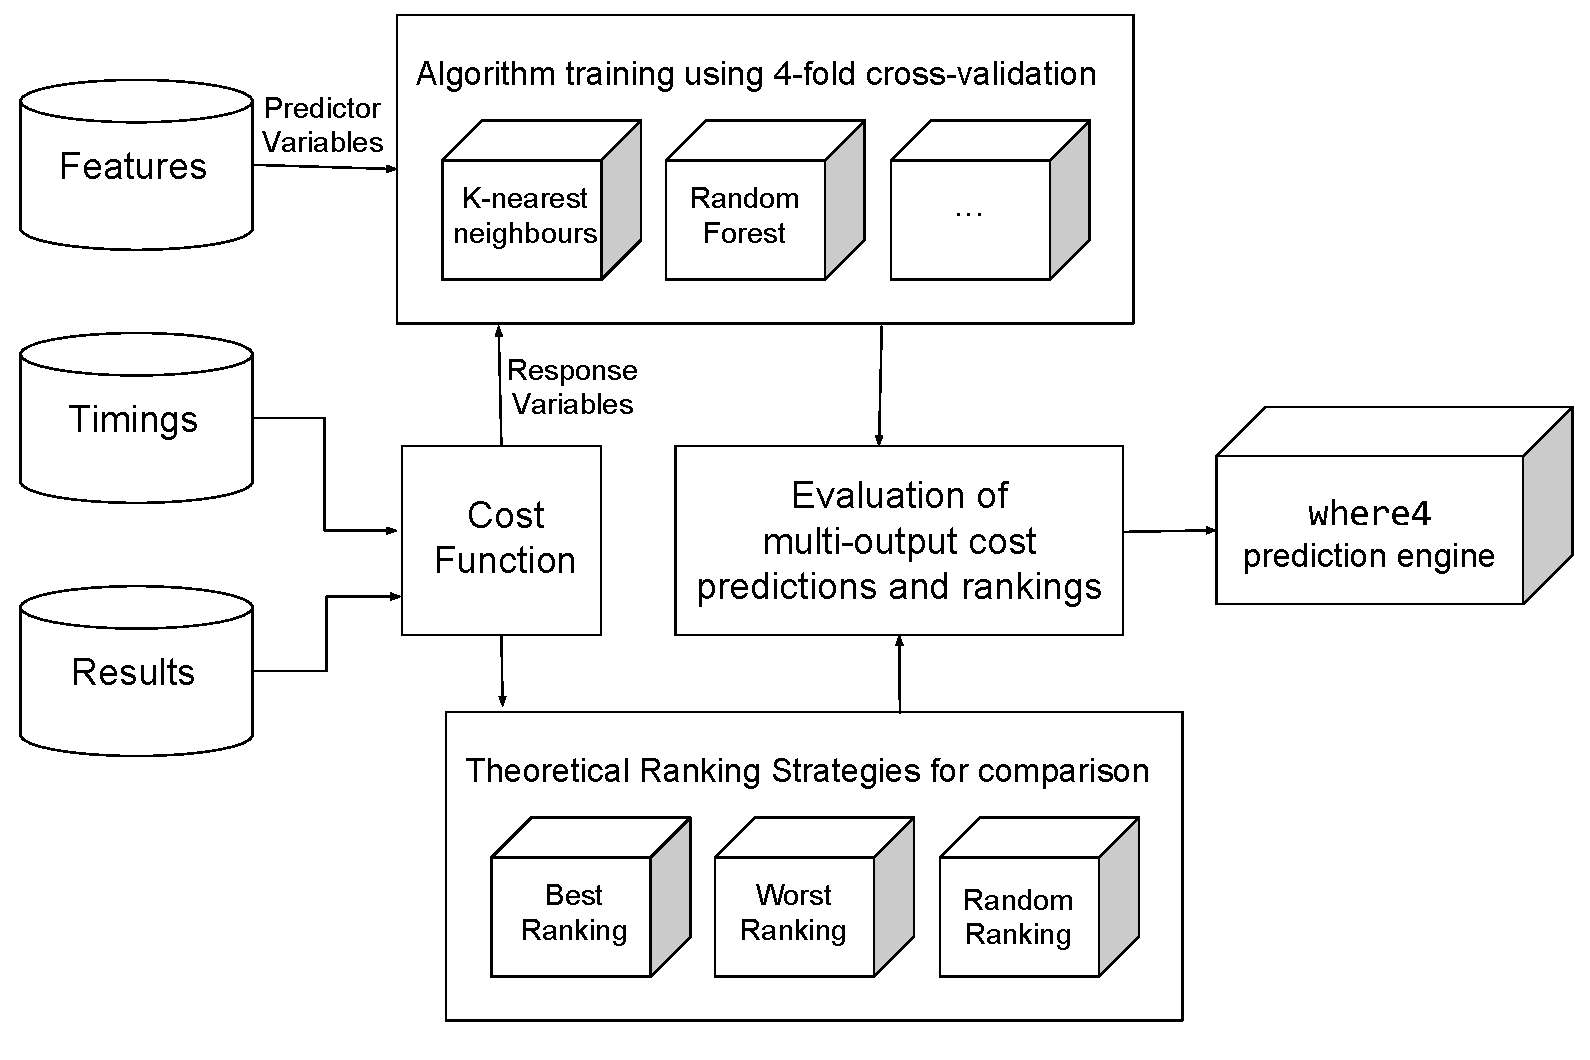
\includegraphics[width=0.9\linewidth]{Figures/Chapter4}
\caption{Overview of the process used to derive the \where4 prediction model}
\label{fig:Chapter4}
\end{figure}


\section{Regression and Classification}

\subsection{The Scoring Function}
% the 'relative utility' of each solver response
\label{sub:scoring}

\section{Introducing three theoretical ranking strategies}
\subsection{Best}
\subsection{Random}
\subsection{Worst}


\section{Choosing the most effective algorithm}
\label{pred:choosing}

\subsection{Normalised Distributed Cumulative Gain}
\subsection{Mean Average Error}
%\subsection{The prediction of score as a regression task}
%\subsection{The prediction of \textit{result} as a classification task}
%\subsection{The prediction of \textit{time} as a regression task}
%\subsection{The prediction of \textit{time} as a classification task}
%\subsubsection{Binarization}
%\subsubsection{Multiclass via binning}
%\subsection{The prediction of score as an ensemble task}
%\subsection{The prediction of score as a multi-label task} 
\subsection{Properties of multi-output problems}
\label{sub:multi}

